\chapter{Realizability}
\label{chap:realizability}%
\chapintro{This chapter is based on results published in~\cite{LohmannW_2009_wsfm}.}


\lettrine[findent=.2em,lines=2,nindent=0pt]{C}{horeographies} which were modeled in a bottom-up approach by composing existing services (also called interconnected models) were investigated in Part~\acronym{II}. In chapters~\ref{chap:verification} and \ref{chap:correction}, we demonstrated how the composition of locally correct (\ie, controllable) services can introduce subtle errors such as deadlocks. Using model checking and strategy synthesis techniques, these errors can be automatically detected and\,---\,to some extent\,---\,corrected.

The converse of the bottom-up approach is the top-down approach which tries to avoid these problems in the first place by creating a service composition out of a choreography specification, called interaction model. This service composition is then \emph{compatible by design}. A choreography specification describes the interaction from a global point of view without specifying unnecessary details about the internal control flow of the involved parties. In any case, there is no distinguished coordinator as it is the case in an orchestration setting.

Several languages have been proposed for specifying choreographies (\citet{SuBFZ_2007_wsfm} provide a survey). They all have in common that they permit to specify unreasonable interactions. An example for a potentially unreasonable interaction is to require that a message from participant~$A$ to participant~$B$ must be exchanged before another message from~$C$ to~$D$. As long as no other messages are passed between~$A$ and~$C$ or~$B$ and~$C$ this requirement cannot be satisfied. For distinguishing between reasonable and unreasonable interaction, the concept of \emph{realizability}~\cite{FuBS_2004_tcs,AlurEY_2003_tse} was introduced. Intuitively, realizability describes the dilemma of balancing compliance with the global specification on the one hand and flexibility and autonomy of the participating services on the other hand.

In this chapter, we address the following \emph{issues} in existing approaches to choreographies and realizability notions. \emph{First}, several approaches only focus on synchronous interaction: asynchronous interaction is either not considered at all, or is brought into the approach as a derivative of the synchronous approach. For instance, several approaches specify only the order in which messages are sent, but leave the order in which they should be received open. Consequently, we employ service automata for modeling choreographies where \emph{synchronous and asynchronous communications are both first-class citizens}. In our setting, causality between the receipt of a message and sending another one can be specified.

\emph{Second}, there appear to be several proposals for defining realizability. Consequently, we propose a \emph{hierarchy} of realizability notions which includes and extends existing concepts.

Controllability asks whether a given service has compatible partners. Existing techniques for answering the controllability problem are capable of synthesizing a compatible partner if it exists. Hence, {\em third}, we suggest techniques to synthesize internals of realizing partners. By relating the realizability problem to controllability, we, {\em fourth}, get the opportunity to study specifications which involve both a choreography and the specification of the internal behavior of some of the participants. This way, we marry the choreography approach with the orchestration approach as well as interaction models with interconnected models. Both approaches have so far been conceived as complementary paradigms for building up complex processes from services~\cite{Peltz_2003_ieee,DijkmanD_2004_ijcis}.

\medskip

The remainder of this chapter is organized as follows. In the next section, we show how service automata can be used to model choreographies. In \autoref{sect:realizability_realizability}, we recall different realizability notions and introduce the novel concept of \emph{distributed realizability}, which is more liberal than complete realizability, yet stricter than partial realizability and hence complements the existing notions. The main contribution is presented in \autoref{sect:realizing_choreographies}: the realizability problem can be approached with algorithms from controllability. \Autoref{sect:realizability_asynchron} is dedicated to issues arising in case asynchronous communication is considered. In \autoref{sect:realizability_application}, we show how the relationship between controllability and realizability can be used to combine aspects from interaction modeling and interconnected models. \Autoref{sect:realizability_related} discusses related work, and \autoref{sect:realizability_conclusion} concludes and gives directions for future research.





%%%%%%%%%%%%%%%%%%%%%%%%%%%%%%%%%%%%%%%%%%%%%%%%%%%%%%%%%%%%%%%%%%%%%%%%%%%%%%%
\section{Modeling choreographies}
\label{sect:realizability_framework}
%%%%%%%%%%%%%%%%%%%%%%%%%%%%%%%%%%%%%%%%%%%%%%%%%%%%%%%%%%%%%%%%%%%%%%%%%%%%%%%

A choreography specification usually consists of two parts: First, a description of the participants and the message channels between them (\ie, the structure or syntax of the choreography, called \emph{collaboration}); and second, a specification of the desired interactions between these participants (\ie, the semantics of the choreography). The former, structural, aspects of a choreography can be expressed by sets of ports.

%%%%%%%%%%%%%%%%%%%%%%%%%%%%%%%%%%%%%%%%%%%%%%%%%%%%%%%%%%%%%%%%%%%%%%%%%%%%%%
\begin{definition}{Peer, collaboration}
A \emph{peer} is a set $\mathcal{P}=\{[I_{1},O_{1}],\ldots,[I_{n},O_{n}]\}$ of ports such that (1) $I_{i}\cap O_{i}=\emptyset$ for all $i$ and (2) $(I_{i}\cup O_{i})\cap (I_{j}\cup O_{j})=\emptyset$ for all $i\neq j$. A \emph{collaboration} is a set $\{\mathcal{P}_{1},\ldots,\mathcal{P}_{m}\}$ of peers such that $\bigcup_{i=1}^{m} \mathcal{P}_{i}$ is a closed interface.
\end{definition}
%%%%%%%%%%%%%%%%%%%%%%%%%%%%%%%%%%%%%%%%%%%%%%%%%%%%%%%%%%%%%%%%%%%%%%%%%%%%%%

A \emph{peer} consists of a set of ports whose message channels are pairwise disjoint. These shall be later implemented by a service automaton. We need to employ \emph{sets} of ports to express situations in which one participant communicates with \emph{several} other services using several ports. \Autoref{fig:peerport} illustrates this.

%%%%%%%%%%%%%%%%%%%%%%%%%%%%%%%%%%%%%%%%%%%%%%%%%%%%%%%%%%%%%%%%%%%%%%%%%%%%%%
\begin{figure}
\centering
\subfigure[collaboration]{\makebox[0.49\textwidth]{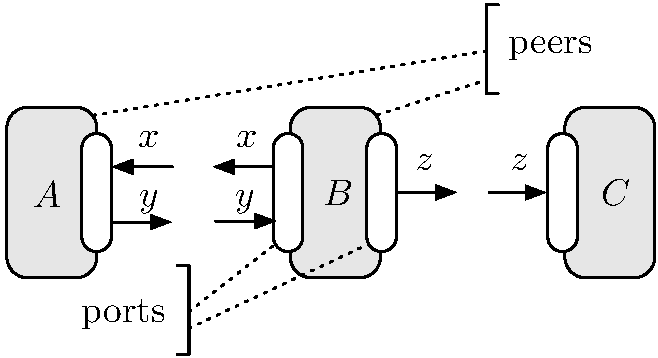
\includegraphics[scale=0.4]{realizability/peerport1}}}
\subfigure[collaboration (shorthand notation)]{\makebox[0.49\textwidth]{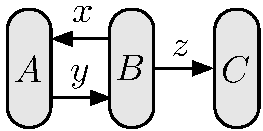
\includegraphics[scale=0.4]{realizability/peerport2}}}
\caption{Illustration of the role of peers and ports in a collaboration.}\label{fig:peerport}
\end{figure}
%%%%%%%%%%%%%%%%%%%%%%%%%%%%%%%%%%%%%%%%%%%%%%%%%%%%%%%%%%%%%%%%%%%%%%%%%%%%%%

As the union of the peers form a closed interface, a closed multiport service automaton can be used as a formal model for the behavior of a choreography. This ensures a closed world (cf.\ \autoref{def:interface}) and bilateral communication between the participants (\ie, each message has exactly one sender and one receiver). At the same time, a closed service automaton implicitly defines a set of runs.

%%%%%%%%%%%%%%%%%%%%%%%%%%%%%%%%%%%%%%%%%%%%%%%%%%%%%%%%%%%%%%%%%%%%%%%%%%%%%%
\begin{definition}{Conversation, choreography}%
\nomenclature[s1]{$\sigma$}{a run of a closed service automaton}%
\nomenclature[s11]{$\sigma_{\mid\E}$}{a run of a closed service automaton without $\tau$-steps}%
\nomenclature[LA]{$\mathcal{L}(A)$}{the language of the closed service automaton $A$}%
\nomenclature[#]{$\#_{x}(\sigma)$}{the number of occurrences $x$ in the run $\sigma$}%
Let $\mathcal{C}=\{\mathcal{P}_{1},\ldots,\mathcal{P}_{n}\}$ be a collaboration and $A=[Q,q_{0},{\shortrightarrow},\Omega,\bigcup \mathcal{C}]$ be a closed service automaton. A maximal terminating run $\sigma$ of $A$ is a \define{conversation} if no $\tau$-transition occurs in $\sigma$ and, for all $x\in \M_{a}$,
$\#_{!x}(\sigma)=\#_{?x}(\sigma)$ and for every prefix $\sigma'$ of $\sigma $ holds: $\#_{!x}(\sigma')\geq\#_{?x}(\sigma')$. Thereby, $\#_{x}(\sigma)$ denotes the number of occurrences of the message event $x$ in the run $\sigma$. A \define{choreography} is a set of conversations.

For a run $\sigma$, define the \define{event sequence} of $\sigma$ as $\sigma|_{\E}$ (\ie, $\sigma$ without $\tau$-steps). The \define{language} of $A$, denoted $\mathcal{L}(A)$, is the union of the event sequences of all runs of~$A$. $A$~is a \define{choreography automaton}, if $A$ is deterministic and $\tau$-free, and $\mathcal{L}(A)$ is a choreography.\label{def:realizability_choreography}
\end{definition}
%%%%%%%%%%%%%%%%%%%%%%%%%%%%%%%%%%%%%%%%%%%%%%%%%%%%%%%%%%%%%%%%%%%%%%%%%%%%%%

The requirements for a conversation state that asynchronous events are always paired (messages do not get lost), and a send event always occurs before the respective receive event. Synchronous communication is not restricted. Conversations are defined in terms of terminating runs (cf.\ \autoref{def:run}) which is similar to \emph{well-behaved} runs defined by \citet{BultanFF_2009_icws}.

In this thesis, we define choreographies as a set of \emph{message event sequences}, which complies with the common understanding of choreographies~\cite{Peltz_2003_ieee,BultanFHS_2003_www,w3c_2003_glossary}. We are aware of proposals to additionally model \emph{local} choices~\cite{DeckerW_2007_bpm} or \emph{internal} behavior in a choreography~\cite{KoppL_2009_zeus}. This, however, contradicts our understanding that a choreography is a \emph{global} specification of the \emph{interaction behavior} of a service composition. Keeping internals secret may have several reasons. On one hand, trade secrets may be involved as the parties may be competitors. On the other hand, an internal control flow may not exist in case the choreography is specified in a design-by-contract scenario.

A mapping from existing interaction modeling languages such as interaction Petri nets~\cite{DeckerW_2007_bpm}, Let's Dance~\cite{ZahaBDH_2006_otm}, message sequence charts~\cite{AlurEY_2003_tse}, collaboration diagrams~\cite{BultanF_2008_soca}, i\acronym{BPMN}~\cite{DeckerB_2007_bpmw}, or \acronym{BPMN} 2.0 choreographies~\cite{standard_bpmn2} to choreography automata is straightforward. Whereas these languages differ in syntax and semantics, concepts such as an underlying collaboration (\ie, the set of ports), the choreography (\ie, the intended global behavior) can be easily derived from these languages. \Autoref{fig:realizability_example} depicts different models specifying the same choreography.

%%%%%%%%%%%%%%%%%%%%%%%%%%%%%%%%%%%%%%%%%%%%%%%%%%%%%%%%%%%%%%%%%%%%%%%%%%%%%%
\begin{figure}[tb]
\centering
\subfigure[choreography automaton\label{fig:realizability_automaton}]{\makebox[0.49\textwidth]{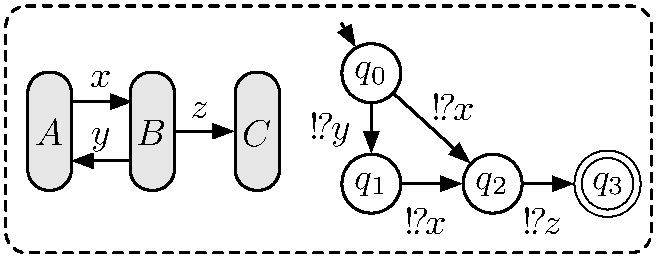
\includegraphics[scale=0.4]{realizability/newchor1}}}
\subfigure[message sequence charts]{\makebox[0.49\textwidth]{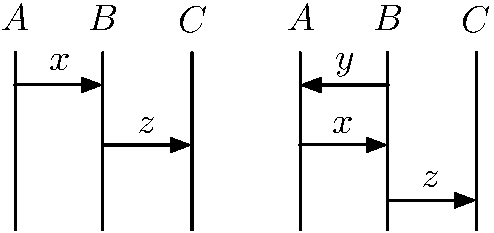
\includegraphics[scale=0.4]{realizability/example-msc}}}\hfill
\subfigure[UML collaboration diagram]{\makebox[0.49\textwidth]{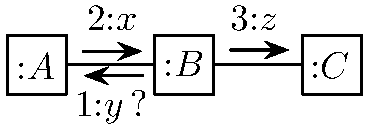
\includegraphics[scale=0.4]{realizability/example-collab}}}
\subfigure[Let's Dance model]{\makebox[0.49\textwidth]{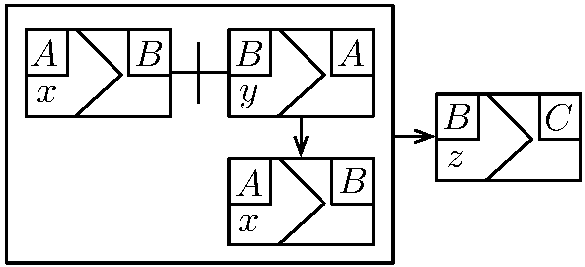
\includegraphics[scale=0.4]{realizability/example-letsdance}}}\hfill
\subfigure[iBPMN model]{\makebox[0.49\textwidth]{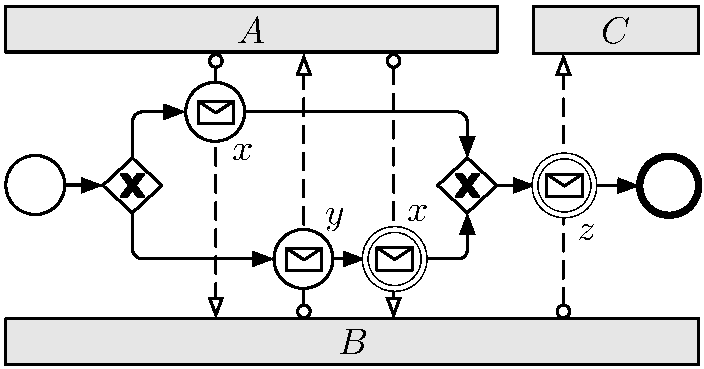
\includegraphics[scale=0.4]{realizability/example-ibpmn}}}\hfill
\subfigure[BPMN 2.0 choreography]{\makebox[0.49\textwidth]{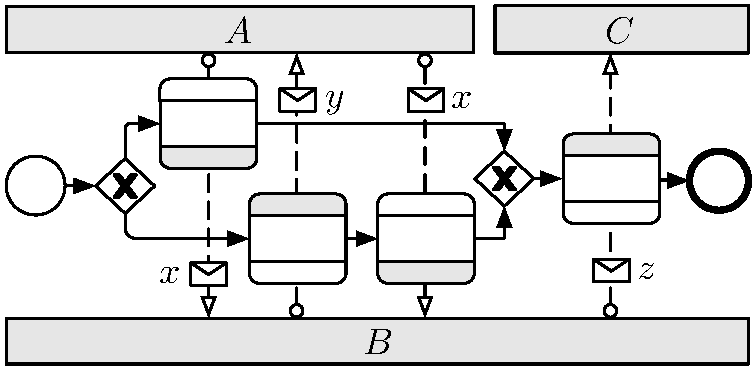
\includegraphics[scale=0.4]{realizability/example-bpmn2}}}
\caption{Different interaction modeling languages specifying the choreography $\{{\sync x\,\sync z}, {\sync y\,\sync x\,\sync z}\}$.}
\label{fig:realizability_example}
\end{figure}
%%%%%%%%%%%%%%%%%%%%%%%%%%%%%%%%%%%%%%%%%%%%%%%%%%%%%%%%%%%%%%%%%%%%%%%%%%%%%%

%%%%%%%%%%%%%%%%%%%%%%%%%%%%%%%%%%%%%%%%%%%%%%%%%%%%%%%%%%%%%%%%%%%%%%%%%%%%%%
\begin{figure}
\centering
\subfigure[dependency violation\label{fig:realizability_violation}]{\makebox[0.49\textwidth]{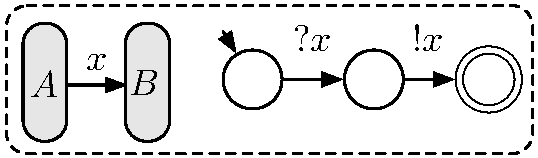
\includegraphics[scale=0.4]{realizability/newchor2}}}\hfill
\subfigure[unbounded message buffer\label{fig:realizability_unbounded}]{\makebox[0.49\textwidth]{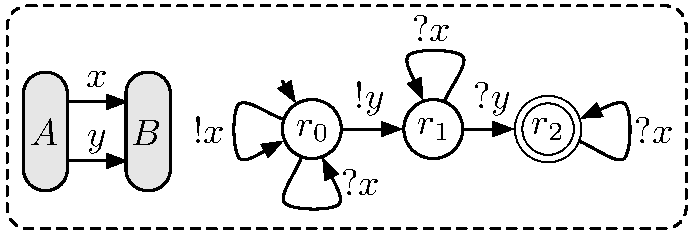
\includegraphics[scale=0.4]{realizability/newchor3}}}
\caption{The multiport service automata (a) and (b) do not specify a choreography.}
\label{fig:realizability_nochor}
\end{figure}
%%%%%%%%%%%%%%%%%%%%%%%%%%%%%%%%%%%%%%%%%%%%%%%%%%%%%%%%%%%%%%%%%%%%%%%%%%%%%%

However, not every $\tau$-free multiport service automaton specifies a choreography. \Autoref{fig:realizability_violation} depicts a service automaton that violates the causal dependency between an asynchronous send and the respective receive event. Another problem arises in settings such as shown in \autoref{fig:realizability_unbounded} in which an arbitrary number of $x$-messages needs to be buffered. In \autoref{sect:realizability_asynchron}, we show how bounded message buffers can be enforced and all runs that are not conversations can be removed from a service automaton.

Finally, not every choreography can be expressed by a multiport service automaton, for example the context-free choreography$$\{({\sync d})^i({\sync e})^i\mid i\in\mathds{N}^{+}\}  = \{{\sync d}\,{\sync e},{\sync d}\,{\sync d}\,{\sync e}\,{\sync e},\dots\}$$ (an example for a Dyck language) cannot be expressed. In this thesis, we only consider regular choreographies, because language equivalence and language containment is undecidable for context-free languages, and hence realizability is undecidable for context-free choreographies.





%%%%%%%%%%%%%%%%%%%%%%%%%%%%%%%%%%%%%%%%%%%%%%%%%%%%%%%%%%%%%%%%%%%%%%%%%%%%%%%
\section{Realizability notions}
\label{sect:realizability_realizability}
%%%%%%%%%%%%%%%%%%%%%%%%%%%%%%%%%%%%%%%%%%%%%%%%%%%%%%%%%%%%%%%%%%%%%%%%%%%%%%%

A choreography specifies the desired global behavior of a service composition. This specification can be interpreted as safety properties (no unspecified conversations are allowed) and liveness properties (every interaction sequence can be completed to a conversation). The composition of service automata, each implementing one peer, can be related to a specified choreography, which leads to the concept of \emph{complete realizability}~\cite{SuBFZ_2007_wsfm,FuBS_2004_tcs,AlurEY_2003_tse,DeckerW_2007_bpm,BultanF_2008_soca,Decker_2009_zeus,Decker_2009_phd} (sometimes called ``full realizability'' or just ``realizability'').

%%%%%%%%%%%%%%%%%%%%%%%%%%%%%%%%%%%%%%%%%%%%%%%%%%%%%%%%%%%%%%%%%%%%%%%%%%%%%%
\begin{definition}{Complete realizability}%
Let $\mathcal{C}=\{\mathcal{P}_{1},\ldots,\mathcal{P}_{n}\}$ be a collaboration and $A$ a choreography automaton implementing the set of ports $\bigcup \mathcal{C}$. The composable service automata $A_{1},\ldots,A_{n}$ \define{completely realize}~$A$ if, for all $i$, $A_{i}$ implements the set of ports $\mathcal{P}_{i}$ and $\mathcal{L}(A_{1}\oplus\cdots\oplus A_{n})=\mathcal{L}(A)$.%
\label{def:realizability_completerealizability}%
\end{definition}
%%%%%%%%%%%%%%%%%%%%%%%%%%%%%%%%%%%%%%%%%%%%%%%%%%%%%%%%%%%%%%%%%%%%%%%%%%%%%%

Complete realizability is a strong requirement, because it demands that the observable behavior of the participants exactly matches the choreography. That is, all safety and liveness properties must be satisfied. In practice, it is often the case that not all aspects of a choreography can be implemented. To this end, \citet{ZahaDHBD_2006_edoc} introduce the  notion \emph{local enforceability} (also called \emph{partial realizability} or \emph{weak realizability}), which only demands that a subset of the choreography is realized by the participants:

%%%%%%%%%%%%%%%%%%%%%%%%%%%%%%%%%%%%%%%%%%%%%%%%%%%%%%%%%%%%%%%%%%%%%%%%%%%%%%
\begin{definition}{Partial realizability}%
Let $\mathcal{C}=\{\mathcal{P}_{1},\ldots,\mathcal{P}_{n}\}$ be a collaboration and $A$ a choreography automaton implementing the set of ports $\bigcup \mathcal{C}$. The composable service automata $A_{1},\ldots,A_{n}$ \define{partially realize} $A$ if, for all $i$, $A_{i}$ implements the set of ports $\mathcal{P}_{i}$ and $\emptyset\neq\mathcal{L}(A_{1}\oplus\cdots\oplus A_{n})\subseteq\mathcal{L}(A)$.
\end{definition}
%%%%%%%%%%%%%%%%%%%%%%%%%%%%%%%%%%%%%%%%%%%%%%%%%%%%%%%%%%%%%%%%%%%%%%%%%%%%%%

Partial realizability requires all safety properties to hold, but makes no assumption on liveness properties other than demanding the set of realized conversations is not empty. Obviously, complete realizability implies partial realizability. Though this weaker notion ensures that all constraints of the choreography are satisfied, it still only considers a single tuple of service automata. If there does not exist such a tuple of automata that realizes the \emph{complete} choreography, there may still exist a \emph{set} of tuples\,---\,each partially realizing the choreography\,---\,which \emph{distributedly} realizes the complete choreography:

%%%%%%%%%%%%%%%%%%%%%%%%%%%%%%%%%%%%%%%%%%%%%%%%%%%%%%%%%%%%%%%%%%%%%%%%%%%%%%
\begin{definition}{Distributed realizability}%
Let $\mathcal{C}=\{\mathcal{P}_{1},\ldots,\mathcal{P}_{n}\}$ be a collaboration and $A$ a choreography automaton implementing the set of ports $\bigcup \mathcal{C}$. The tuples of service automata $[A_{1}^{1},\ldots,A_{n}^{1}],\ldots,$ $[A_{1}^{m},\ldots,A_{n}^{m}]$ \define{distributedly realize} $A$ if, for $i=1,\ldots,n$ and $j=1,\ldots,m$,
\begin{myenumerate}
\item $A_{i}^{j}$ implements the set of ports $\mathcal{P}_{i}$,
\item $A_{1}^{j},\ldots, A_{n}^{j}$ are composable,
\item $\emptyset\neq\mathcal{L}(A_{1}^{j}\oplus\cdots\oplus A_{n}^{j})\subseteq \mathcal{L}(A)$, and
\item $\bigcup_{j=1}^m \mathcal{L}(A_{1}^{j}\oplus\cdots\oplus A_{n}^{j}) = \mathcal{L}(A)$.
\end{myenumerate}
\end{definition}
%%%%%%%%%%%%%%%%%%%%%%%%%%%%%%%%%%%%%%%%%%%%%%%%%%%%%%%%%%%%%%%%%%%%%%%%%%%%%%

Distributed realizability allows for design-time coordination between participants: From a set of different possible implementations, we can choose a specific tuple of implementations which are coordinated in the sense that each participant can rely on the other participant's behavior. In addition, every conversation specified by the choreography can be realized by at least one tuple of implementing service automata; that is, the choreography does not contain ``dead code'' which would be unusable by any partner set. Although it is a stronger notion than partial realizability (\ie, more of the choreography's behavior is implemented), it is still a weaker notion than complete realizability. \Autoref{fig:realizability:visualization} illustrates the different notions.

%%%%%%%%%%%%%%%%%%%%%%%%%%%%%%%%%%%%%%%%%%%%%%%%%%%%%%%%%%%%%%%%%%%%%%%%%%%%%%
\begin{figure}
\centering
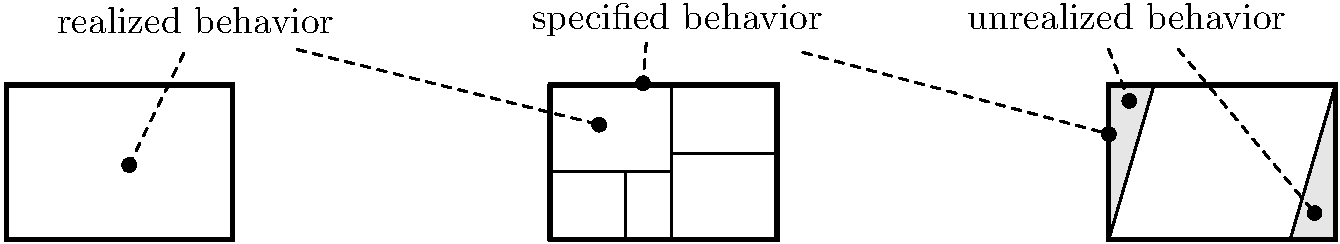
\includegraphics[scale=0.4]{realizability/boxes}\vspace{-1em}\\
\hfill
\subfigure[complete realizability]{\makebox[0.3\textwidth]{}}\hfill
\subfigure[distributed realizability]{\makebox[0.35\textwidth]{}}\hfill
\subfigure[partial realizability]{\makebox[0.3\textwidth]{}}\hfill{$\empty$}
\caption{Visualization of realizability notions.}\label{fig:realizability:visualization}
\end{figure}
%%%%%%%%%%%%%%%%%%%%%%%%%%%%%%%%%%%%%%%%%%%%%%%%%%%%%%%%%%%%%%%%%%%%%%%%%%%%%%

%%%%%%%%%%%%%%%%%%%%%%%%%%%%%%%%%%%%%%%%%%%%%%%%%%%%%%%%%%%%%%%%%%%%%%%%%%%%%%
\begin{figure}[tb]
\centering
\subfigure[completely realizable choreography]{\makebox[0.49\textwidth]{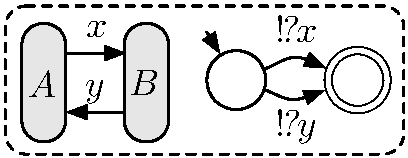
\includegraphics[scale=0.4]{realizability/newchor4}}}\hfill
\subfigure[a pair of realizing participants]{\makebox[0.49\textwidth]{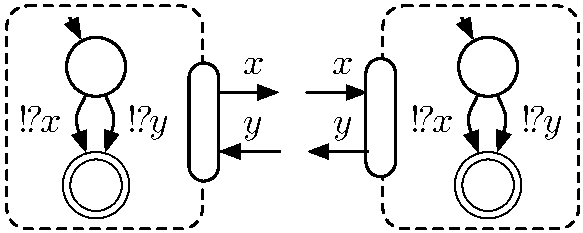
\includegraphics[scale=0.4]{realizability/real1}}}\\
\subfigure[distributedly realizable choreography]{\makebox[0.49\textwidth]{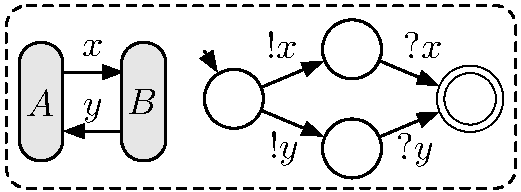
\includegraphics[scale=0.4]{realizability/newchor5}}}\hfill
\subfigure[two tuples of realizing participants]{\makebox[0.49\textwidth]{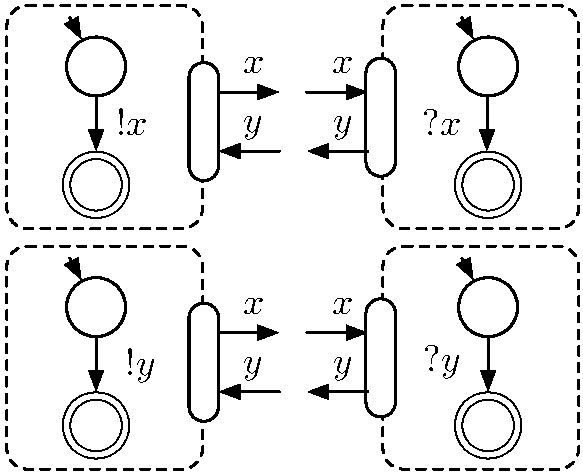
\includegraphics[scale=0.4]{realizability/real23}}}\\
\subfigure[partially realizable choreography]{\makebox[0.49\textwidth]{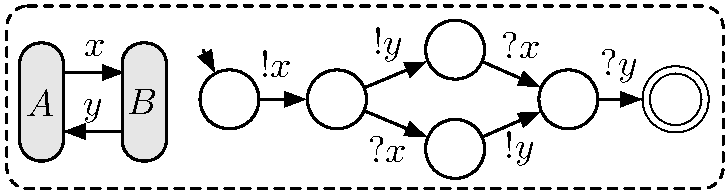
\includegraphics[scale=0.4]{realizability/newchor6}}}\hfill
\subfigure[a pair of realizing participants]{\makebox[0.49\textwidth]{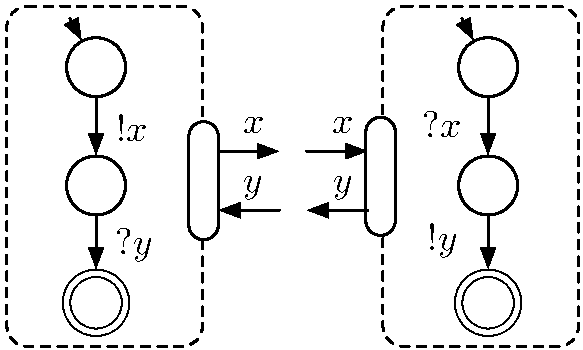
\includegraphics[scale=0.4]{realizability/real4}}}
\caption{The choreography (a) is completely realizable, (c) is distributedly realizable, and (e) is partially realizable.}
\label{fig:realizability_hierarchy}
\end{figure}
%%%%%%%%%%%%%%%%%%%%%%%%%%%%%%%%%%%%%%%%%%%%%%%%%%%%%%%%%%%%%%%%%%%%%%%%%%%%%%


\paragraph{Example.}

Consider the choreographies in \autoref{fig:realizability_hierarchy}.
The choreography in which the participants communicate synchronously~(a) is completely realizable by a set of service automata~(b) which synchronize at runtime via message~$x$ or $y$. In case the messages are sent asynchronously~(c), this is no longer possible. This choreography is not completely realizable, because there does not exist a single pair of service automata which implements the specified behavior. However, the implementations can be coordinated at design time: either participant~$A$ sends a message and participant~$B$ is quiet or the other way around~(d). These two pairs distributedly realize the whole choreography. Finally, choreography~(e) can only be partially realized, because the conversation ${!x!y?x?y}$ cannot be implemented by the participants without also producing the unspecified conversations ${!y!x?x?y}$ or ${!y!x?y?x}$. However, the conversation ${!x?x!y?y}$ can be realized~(f).





%%%%%%%%%%%%%%%%%%%%%%%%%%%%%%%%%%%%%%%%%%%%%%%%%%%%%%%%%%%%%%%%%%%%%%%%%%%%%%
\section{Realizing choreographies}
\label{sect:realizing_choreographies}
%%%%%%%%%%%%%%%%%%%%%%%%%%%%%%%%%%%%%%%%%%%%%%%%%%%%%%%%%%%%%%%%%%%%%%%%%%%%%%%

In this section, we show how the different notions of realizability can be checked and how a realizable choreography can be projected to implementing service automata. A close relationship to a controllability notion allows us to use an existing algorithm to remove unrealizable behavior from choreographies.




%%%%%%%%%%%%%%%%%%%%%%%%%%%%%%%%%%%%%%%%%%%%%%%%%%%%%%%%%%%%%%%%%%%%%%%%%%%%%%
\subsection*{Projection and independence}

The tuples of service automata which realize a choreography are existentially quantified in the definitions of the different realizability notions. To this end, realizability can be seen as a synthesis problem: given the choreography specification, we are interested in realizing peer implementations. As the choreography describes the global behavior of all peers, it can be used as a starting point to \emph{project} this global behavior to the different peers.

As discussed earlier, the different realizability notions differ in the amount of conversations which must be realized by the peers. They all have in common that no new conversation must be introduced. Hence, the projected peers need to be \emph{coordinated} at design time such that they do not produce unspecified conversations. The example choreographies in \autoref{fig:realizability_hierarchy} showed that this coordination can already be impossible even if two peers share message channels. To characterized possible and impossible coordination, we first introduce \emph{distant} message events. We call two message events distant if there exists no peer which can observe both:

%%%%%%%%%%%%%%%%%%%%%%%%%%%%%%%%%%%%%%%%%%%%%%%%%%%%%%%%%%%%%%%%%%%%%%%%%%%%%%
\begin{definition}{Distant message events}%
Let $\mathcal{C}=\{\mathcal{P}_{1},\ldots,\mathcal{P}_{n}\}$ be a collaboration. Two message events $a,b\in \E$ are \emph{distant} iff there exist no peer $\mathcal{P}\in \mathcal{C}$ such that $\{a,b\}\subseteq \E_{{}\bigcup \mathcal{P}}$.
\end{definition}
%%%%%%%%%%%%%%%%%%%%%%%%%%%%%%%%%%%%%%%%%%%%%%%%%%%%%%%%%%%%%%%%%%%%%%%%%%%%%%

Distant message events cannot be coordinated by any peer. There only exist two scenarios in which distant message events do not jeopardize realizability: either they can be removed from the choreography without resulting in an empty set of conversations, or they do not need to be coordinated in the first place. Whereas the former setting results in implementations which do not completely realize the choreography, message events enjoying the latter property are called \emph{independent}. Informally, two events are independent if they (1) neither activate (2) nor deactivate each other, and (3) if they occur in one specific order reaching a state $q$, then any other ordering must be possible, possibly reaching a different state $q'$, which, however, must be equivalent to $q$.

%%%%%%%%%%%%%%%%%%%%%%%%%%%%%%%%%%%%%%%%%%%%%%%%%%%%%%%%%%%%%%%%%%%%%%%%%%%%%%
\begin{definition}{Independence~\cite{Wolf_2008_topnoc}}%
Let $\mathcal{C}=\{\mathcal{P}_{1},\ldots,\mathcal{P}_{n}\}$ be a collaboration, $A=[Q,q_{0},{\shortrightarrow},\Omega,\bigcup\mathcal{C}]$ be a $\tau$-free multiport service automaton, and $a,b\in \E$ be distant message events.
\begin{itemize}
\item $a$ \define{activates} $b$ in $q\in Q$, if (1) there exist states $q_{a},q_{ab}\in Q$ with \smash{$q\xrightarrow{a} q_{a}\xrightarrow{b}q_{ab}$}, but there exists no state $q_{b}\in Q$ with \smash{$q\xrightarrow{b} q_{b}$} and (2)~$\M(a)=\M(b)$ implies $a\notin {!\E}$.

\item $a$ \define{disables} $b$ in $q\in Q$, if there exist states $q_{a},q_{b}\in Q$ with \smash{$q\xrightarrow{a} q_{a}$}, \smash{$q\xrightarrow{b}q_{b}$}, but there exists no state $q_{ab}\in Q$ with \smash{$q_{a}\xrightarrow{b} q_{ab}$}.

\item Two states $q_{1},q_{2}\in Q$ are \define{equivalent} iff $\mathcal{L}([Q,\delta,q_{1},F,\mathcal{P}])=\mathcal{L}([Q,\delta,q_{2},F,\mathcal{P}])$.

\item $a$ and $b$ are \define{independent} iff, for all states $q\in Q$ holds: $a$ neither activates nor disables $b$ in $q$ and, if \smash{$q\xrightarrow{a}q_{a}\xrightarrow{b}q_{ab}$} and \smash{$q\xrightarrow{b}q_{b}\xrightarrow{a}q_{ba}$}, then $q_{ab}$ and $q_{ba}$ are equivalent.
\end{itemize}\label{def:independence}%
\end{definition}
%%%%%%%%%%%%%%%%%%%%%%%%%%%%%%%%%%%%%%%%%%%%%%%%%%%%%%%%%%%%%%%%%%%%%%%%%%%%%%

These independence requirements introduced by~\citet{Wolf_2008_topnoc} are weaker than the \emph{lossless-join} property~\cite{FuBS_2004_tcs} and the \emph{well-informed} property~\cite{BultanF_2008_soca} which both aim at complete realizability only. They are, however, similar the \emph{autonomous property}~\cite{FuBS_2004_tcs}.

The second requirement of the definition of activation is an extension of the original definition: \citet{Wolf_2008_topnoc} investigates independence of the states of a most-permissive strategy. There, each state has all possible asynchronous receiving events\,---\,possibly leading to the empty state (see \autoref{sect:strategy}). Hence, an asynchronous send event $!{x}$ would never activate a subsequent asynchronous receive event $?{x}$. The second requirement rules out such scenarios for choreography automata.

If all distant events of a choreography are independent, the choreography can be safely projected to the peers, resulting in a tuple of service automata which realize the choreography.

%%%%%%%%%%%%%%%%%%%%%%%%%%%%%%%%%%%%%%%%%%%%%%%%%%%%%%%%%%%%%%%%%%%%%%%%%%%%%%
\begin{definition}{Participant projection}
\label{def:realizability_projection}%
\nomenclature[AP]{$A{\mid}_{\mathcal{P}}$}{projection of choreography $A$ to port $\mathcal{P}$}%
Let $\mathcal{C}=\{\mathcal{P}_{1},\ldots,\mathcal{P}_{n}\}$ be a collaboration and $A=[Q,q_{0},{\shortrightarrow},\Omega,\bigcup\mathcal{C}]$ be a $\tau$-free multiport service automaton. Define the \define{projection} of $A$ to the peer $\mathcal{P}_{i}$, denoted $A|_{\mathcal{P}_{i}}$, as the service automaton $[Q',q_{0}',{\shortrightarrow}',\Omega',\mathcal{P}_{i}]$ with the initial state $q_{0}':=\project_{\mathcal{P}_{i}}(\{q_{0}\})$ and $Q'$, ${\shortrightarrow}'$, and $\Omega'$ inductively defined as follows:
\begin{itemize}
\item $q_{0}'\in Q'$.
\item If $q\in Q'$ with $q_{1}\in q$, \smash{$q_{1}\xrightarrow{x}q_{2}$}, and $x\in \bigcup \mathcal{P}_{i}$, then $q'\in Q'$ with $q':=\project_{\mathcal{P}_{i}}(\{q_{2}\})\in Q'$ and $[q,x,q']\in{\shortrightarrow}'$. $q'\in \Omega'$ iff $q'\cap \Omega\neq\emptyset$.
\end{itemize}
Thereby, define $\project_{\mathcal{P}_{i}}(S):=\{q'\mid q\in S, \smash{q\xrightarrow{x_{1}}\cdots \xrightarrow{x_{n}} q'}, x_{i}\notin \bigcup \mathcal{P}_{i}\}$ for a set of states $S\subseteq Q$.
\end{definition}
%%%%%%%%%%%%%%%%%%%%%%%%%%%%%%%%%%%%%%%%%%%%%%%%%%%%%%%%%%%%%%%%%%%%%%%%%%%%%%

The set $\project_{\mathcal{P}_{i}}(S)$ contains all states reachable with a (possibly empty) sequence from a state of $S$ which does not contain an event from $\bigcup \mathcal{P}_{i}$. The definition an adaption of the $\closure$ operation (cf.\ \autoref{def:closure}) and was first proposed to be used as a projection algorithm by \citet{Decker_2009_zeus,Decker_2009_phd}.

From \autoref{def:independence} and \autoref{def:realizability_projection} we can conclude:

%%%%%%%%%%%%%%%%%%%%%%%%%%%%%%%%%%%%%%%%%%%%%%%%%%%%%%%%%%%%%%%%%%%%%%%%%%%%%%
\begin{corollary}{Projection of independent choreographies}
Let $\mathcal{C}=\{\mathcal{P}_{1},\ldots,\mathcal{P}_{n}\}$ be a collaboration, $A=[Q,q_{0},{\shortrightarrow},\Omega,\bigcup\mathcal{C}]$ be a choreography automaton such that all distant events are independent.\\ Then $\mathcal{L}(A)=\mathcal{L}(A|_{\mathcal{P}_{1}}\oplus\cdots\oplus A|_{\mathcal{P}_{n}})$.
\end{corollary}
%%%%%%%%%%%%%%%%%%%%%%%%%%%%%%%%%%%%%%%%%%%%%%%%%%%%%%%%%%%%%%%%%%%%%%%%%%%%%%


\paragraph{Example.}

The choreography of \autoref{fig:realizability_automaton}  does not contain distant message events and is completely realizable. \Autoref{fig:real:project} depicts its projection to the peers $A$, $B$, and~$C$.

%%%%%%%%%%%%%%%%%%%%%%%%%%%%%%%%%%%%%%%%%%%%%%%%%%%%%%%%%%%%%%%%%%%%%%%%%%%%%%
\begin{figure}
\centering
\subfigure[peer $A$]{\makebox[0.25\textwidth]{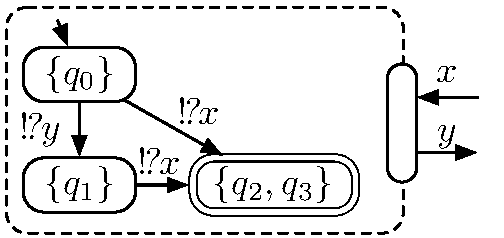
\includegraphics[scale=0.4]{realizability/newproja}}}\hfill
\subfigure[peer $B$]{\makebox[0.49\textwidth]{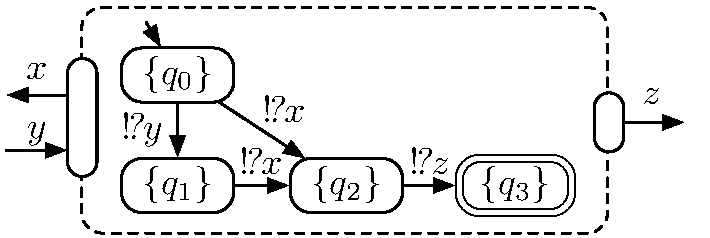
\includegraphics[scale=0.4]{realizability/newprojb}}}\hfill
\subfigure[peer $C$]{\makebox[0.25\textwidth]{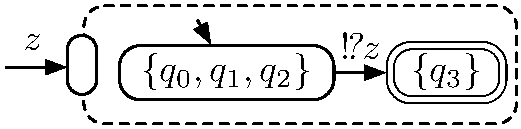
\includegraphics[scale=0.4]{realizability/newprojc}}}
\caption{Choreography projection to service automata.}\label{fig:real:project}
\end{figure}
%%%%%%%%%%%%%%%%%%%%%%%%%%%%%%%%%%%%%%%%%%%%%%%%%%%%%%%%%%%%%%%%%%%%%%%%%%%%%%




%%%%%%%%%%%%%%%%%%%%%%%%%%%%%%%%%%%%%%%%%%%%%%%%%%%%%%%%%%%%%%%%%%%%%%%%%%%%%%
\subsection*{Link to controllability}

\Autoref{def:independence} describes independence in a declarative way. It can be used to \emph{check} whether the events of a choreography are independent. If this is the case, the choreography is completely realizable and \autoref{def:realizability_projection} provides realizing service automata. In case there exist distant events which are not independent, we can only conclude that the choreography is not completely realizable, but we can neither make a statement on the weaker notions of realizability nor can we apply \autoref{def:realizability_projection}.

However, \citet{Wolf_2008_topnoc} not only provides a definition of independence, but also an algorithm to systematically restrict behavior to enforce independence. This algorithm was originally introduced to check a related controllability notion, \emph{decentralized controllability}. Decentralized controllability is an extension of controllability to respect the ports of a service automaton.

%%%%%%%%%%%%%%%%%%%%%%%%%%%%%%%%%%%%%%%%%%%%%%%%%%%%%%%%%%%%%%%%%%%%%%%%%%%%%%
\begin{definition}{Decentralized \boldmath$k$-controllability~\cite{Schmidt_2005_emisa,Wolf_2008_topnoc}}%
Let $A$ be an open multiport service automaton implementing the ports $\{[I_{1},O_{1}],\ldots,[I_{n},O_{n}]\}$. Then $A$ is \define{decentralized $k$-controllable} iff there exists a tuple of single-port service automata $[B_{1},\ldots,B_{n}]$ such that $B_{i}$ implements the port $\{[O_{i},I_{i}]\}$ and $A\oplus B_{1}\oplus\cdots\oplus B_{n}$ is $k$-compatible.
\end{definition}
%%%%%%%%%%%%%%%%%%%%%%%%%%%%%%%%%%%%%%%%%%%%%%%%%%%%%%%%%%%%%%%%%%%%%%%%%%%%%%

In contrast to \autoref{def:controllability}, decentralized controllability takes the ports of~$A$ into account and requires each port to be implemented by a distinct service automaton $B_{i}$. The multiport service automaton $A$ can be seen as an orchestrator for the other service automata. We call $[B_{1},\ldots,B_{n}]$ a \emph{decentralized $k$-strategy} of $A$. Thereby, the single-port service automata $B_{1},\ldots,B_{n}$ only communicate with $A$ and do not share message channels. Hence, they cannot communicate directly with each other during runtime. Only during design time of $B_{1},\ldots,B_{n}$ it is possible to coordinate their behavior.

This setting is similar to the realizability scenario and is related to independence as follows. To synthesize a decentralized strategy, first a ``centralized'' strategy (\ie, a strategy as constructed by \autoref{def:synthesis}) is synthesized. This strategy is an overapproximation of any decentralized strategy, because it serves all ports at once does not require any coordination. This strategy is then ``massaged'' to enforce independency.

To apply the algorithm from~\citet{Wolf_2008_topnoc}, the choreography automaton needs to be made \emph{deterministic}. This is a standard operation for regular automata~\cite{HopcroftMU_1979} and does not restrict generality. It ensures that in every state $q$ and for each event $x$ there is exactly one $x$-labeled edge leaving~$q$. In case such a transition was not specified, the new introduced edge leads to a nonfinal sink state.

\nomenclature[chi]{$\chi$}{global decision event}%

Independency can be achieved by removing those edges and states from the automaton which are dependent. In the case of disabling of events, this removal contains nondeterminism: If, for instance, an event $a$ disables an event $b$ in a state $q$, we can decide to either remove the $a$-successor or the $b$-successor of $q$. This nondeterminism seems to be necessary, as nondeterminism (or backtracking) is one of the few tools to break symmetry~\cite{Schmidt_2005_emisa}. This mutually exclusive deletion yields two different tuples of implementing peers. To avoid restricting the set of local service implementations, we introduce a \emph{global decision event}~$\chi$ in the following definition to express the different outcomes of this nondeterminism. These decision events allow us to postpone the decision which event to remove after the dependency resolution.

%%%%%%%%%%%%%%%%%%%%%%%%%%%%%%%%%%%%%%%%%%%%%%%%%%%%%%%%%%%%%%%%%%%%%%%%%%%%%%
\begin{definition}{Resolution of dependency}
\label{def:realizability_resolution}%
Let $\mathcal{C}=\{\mathcal{P}_{1},\ldots,\mathcal{P}_{n}\}$ be a collaboration, $A=[Q,q_{0},{\shortrightarrow},\Omega,\bigcup\mathcal{C}]$ be a $\tau$-free multiport service automaton, and $a,b\in \E$ be distant message events.
\begin{enumerate}
\item If $a$ disables $b$ in a state $q\in Q$, then introduce two new states $q_{a}$ and $q_{b}$ with \smash{$q\xrightarrow{\chi}q_{a}$}, \smash{$q\xrightarrow{\chi}q_{b}$} such that $q_{a}$ has all outgoing edges of $q$ that are not labeled with $b$ and $q_{b}$ has all outgoing edges of $q$ that are not labeled with $a$. Then remove all outgoing edges of $q$ that are not labeled with $\chi$.
\item If $a$ enables $b$ in a state $q\in Q$, then delete the state $q_{ab}$ with \smash{$q\xrightarrow{a}q_{a}\xrightarrow{b}q_{ab}$}.
\item If the states $q_{ab},q_{ba}\in Q$ with \smash{$q\xrightarrow{a}q_{a}\xrightarrow{b}q_{ab}$} and \smash{$q\xrightarrow{b}q_{b}\xrightarrow{a}q_{ba}$} are not equivalent, then delete $q_{ab}, q_{ba}$ and unite $A$ with the deterministic $\tau$-free multiport service automaton $A'$ with $\mathcal{L}(A')=\mathcal{L}([Q,q_{ab},{\shortrightarrow},\Omega,\mathcal{P}])\cap\mathcal{L}([Q,q_{ba},{\shortrightarrow},\Omega,\mathcal{P}])$ and add the edges \smash{$q_{a}\xrightarrow{b}q_{0}'$} and \smash{$q_{b}\xrightarrow{a}q_{0}'$}.
\end{enumerate}
\end{definition}
%%%%%%%%%%%%%%%%%%%%%%%%%%%%%%%%%%%%%%%%%%%%%%%%%%%%%%%%%%%%%%%%%%%%%%%%%%%%%%

The first step introduces the global decision events if an event is disabled. The second step removes states to avoid the enabling of an event. In the third step, equivalence of states that are reached by different interleavings of events is enforced by intersecting the runs reachable from these states. As we consider regular languages, the automaton having this intersection as language can be constructed easily~\cite{HopcroftMU_1979}.

The original definition of Wolf~\cite{Schmidt_2005_emisa,Wolf_2008_topnoc} is based on acyclic service models. \emph{The algorithm is sound, but not complete: When applied to cyclic models, correctness is guaranteed, but the dependency resolution might not terminate.} A sound and complete algorithm is still subject to future work. We are, however, currently not aware of an example for that \autoref{def:realizability_resolution} does not terminate.

%%%%%%%%%%%%%%%%%%%%%%%%%%%%%%%%%%%%%%%%%%%%%%%%%%%%%%%%%%%%%%%%%%%%%%%%%%%%%%
\begin{figure}
\centering
\subfigure[collaboration]{\makebox[0.3\textwidth]{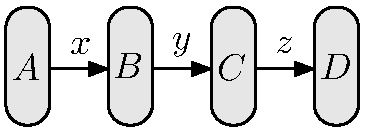
\includegraphics[scale=0.4]{realizability/collaboration5}}}\hfill
\subfigure[the gray states are not equivalent\label{fig:realizability_resolveb}]{\makebox[0.69\textwidth]{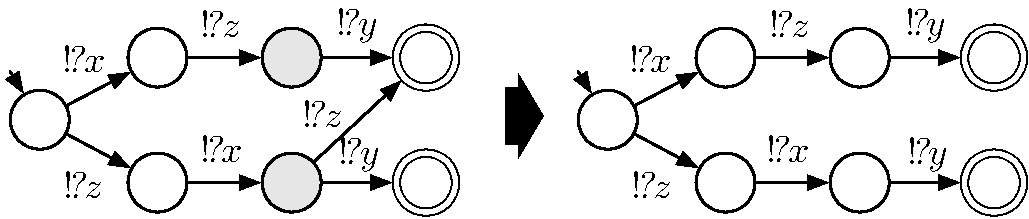
\includegraphics[scale=0.4]{realizability/equivalent}}}
\subfigure[${\sync z}$ enables ${\sync x}$ in the gray state\label{fig:realizability_resolvec}]{\makebox[0.49\textwidth]{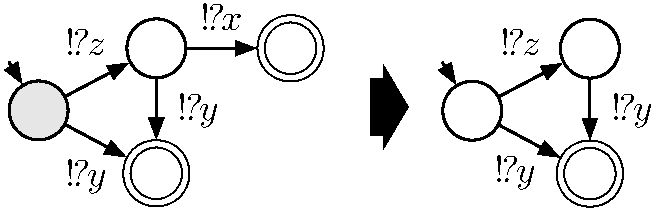
\includegraphics[scale=0.4]{realizability/enable}}}
\subfigure[${\sync x}$ disables ${\sync z}$ in the gray state]{\makebox[0.49\textwidth]{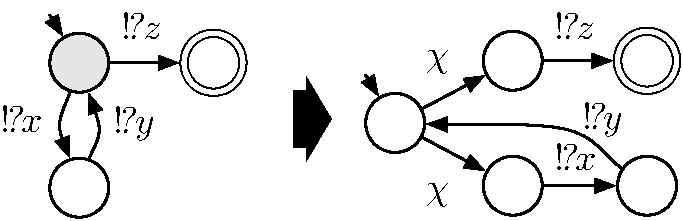
\includegraphics[scale=0.4]{realizability/disable}}}
\caption{Examples for the resolution of dependencies.}
\label{fig:realizability_resolve}
\end{figure}
%%%%%%%%%%%%%%%%%%%%%%%%%%%%%%%%%%%%%%%%%%%%%%%%%%%%%%%%%%%%%%%%%%%%%%%%%%%%%%


\paragraph{Example.}

\Autoref{fig:realizability_resolve}(b)--(d) depict examples for each step. The removal of states and edges can introduce new deadlocks and make other states unreachable from the initial state. Such states need to be removed before projection. A multiport service automaton is\,---\,similar to \autoref{thm:strategy}\,---\,not decentralized controllable iff all states are removed.

\medskip

A multiport service automaton with global decision events such as the example in \autoref{fig:realizability_resolvec} implicitly characterizes a set of multiport service automata in which these decisions have been resolved. Each resolution of these decisions results in a tuple of implementing peers which can be derived using the projection defined in \autoref{def:realizability_projection}. For the example of \autoref{fig:realizability_resolvec}, the global decision is resolved independently each time the initial state is reached. \Autoref{fig:realizability_resolve2} depicts the different resolutions of the global decisions. Each resolution represents a design-time coordination between the peers ${A}$ and ${C}$ on how often the ${\sync x}{\sync y}$ loop should be traversed. As the peers ${A}$ and ${C}$ cannot communicate with each other, this coordination cannot be done during runtime. The set of all possible implementations distributedly realize the choreography.

%%%%%%%%%%%%%%%%%%%%%%%%%%%%%%%%%%%%%%%%%%%%%%%%%%%%%%%%%%%%%%%%%%%%%%%%%%%%%%
\begin{figure}
\centering
\subfigure{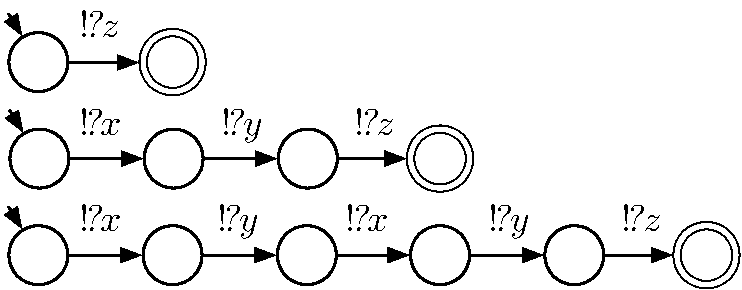
\includegraphics[scale=0.4]{realizability/decide}}
$\qquad\cdots$
\caption{Resolutions of the global decisions in the automaton of \autoref{fig:realizability_resolveb}.}
\label{fig:realizability_resolve2}
\end{figure}
%%%%%%%%%%%%%%%%%%%%%%%%%%%%%%%%%%%%%%%%%%%%%%%%%%%%%%%%%%%%%%%%%%%%%%%%%%%%%%

\medskip

The approach aims at finding the strongest applicable realizability notion. If a state needs to be deleted due to dependencies, we can derive diagnosis information:

\begin{niceitemize}
\item If a state is deleted by step (2) or (3) in~\autoref{def:realizability_resolution}, the choreography is neither completely realizable nor distributedly realizable.

\item If a global decision (\ie, a $\chi$-event) is introduced by step (1), the choreography is not completely realizable, because the considered events are mutually exclusive.

\item If the initial state is removed, the choreography is not partially realizable.
\end{niceitemize}

In any case, the respective state and the events that require state deletion can be used to diagnose the choreography and to introduce messages that restore independency.




%%%%%%%%%%%%%%%%%%%%%%%%%%%%%%%%%%%%%%%%%%%%%%%%%%%%%%%%%%%%%%%%%%%%%%%%%%%%%%
\subsection*{Implementation}

%%%%%%%%%%%%%%%%%%%%%%%%%%%%%%%%%%%%%%%%%%%%%%%%%%%%%%%%%%%%%%%%%%%%%%%%%%%%%%
\begin{figure}
\centering
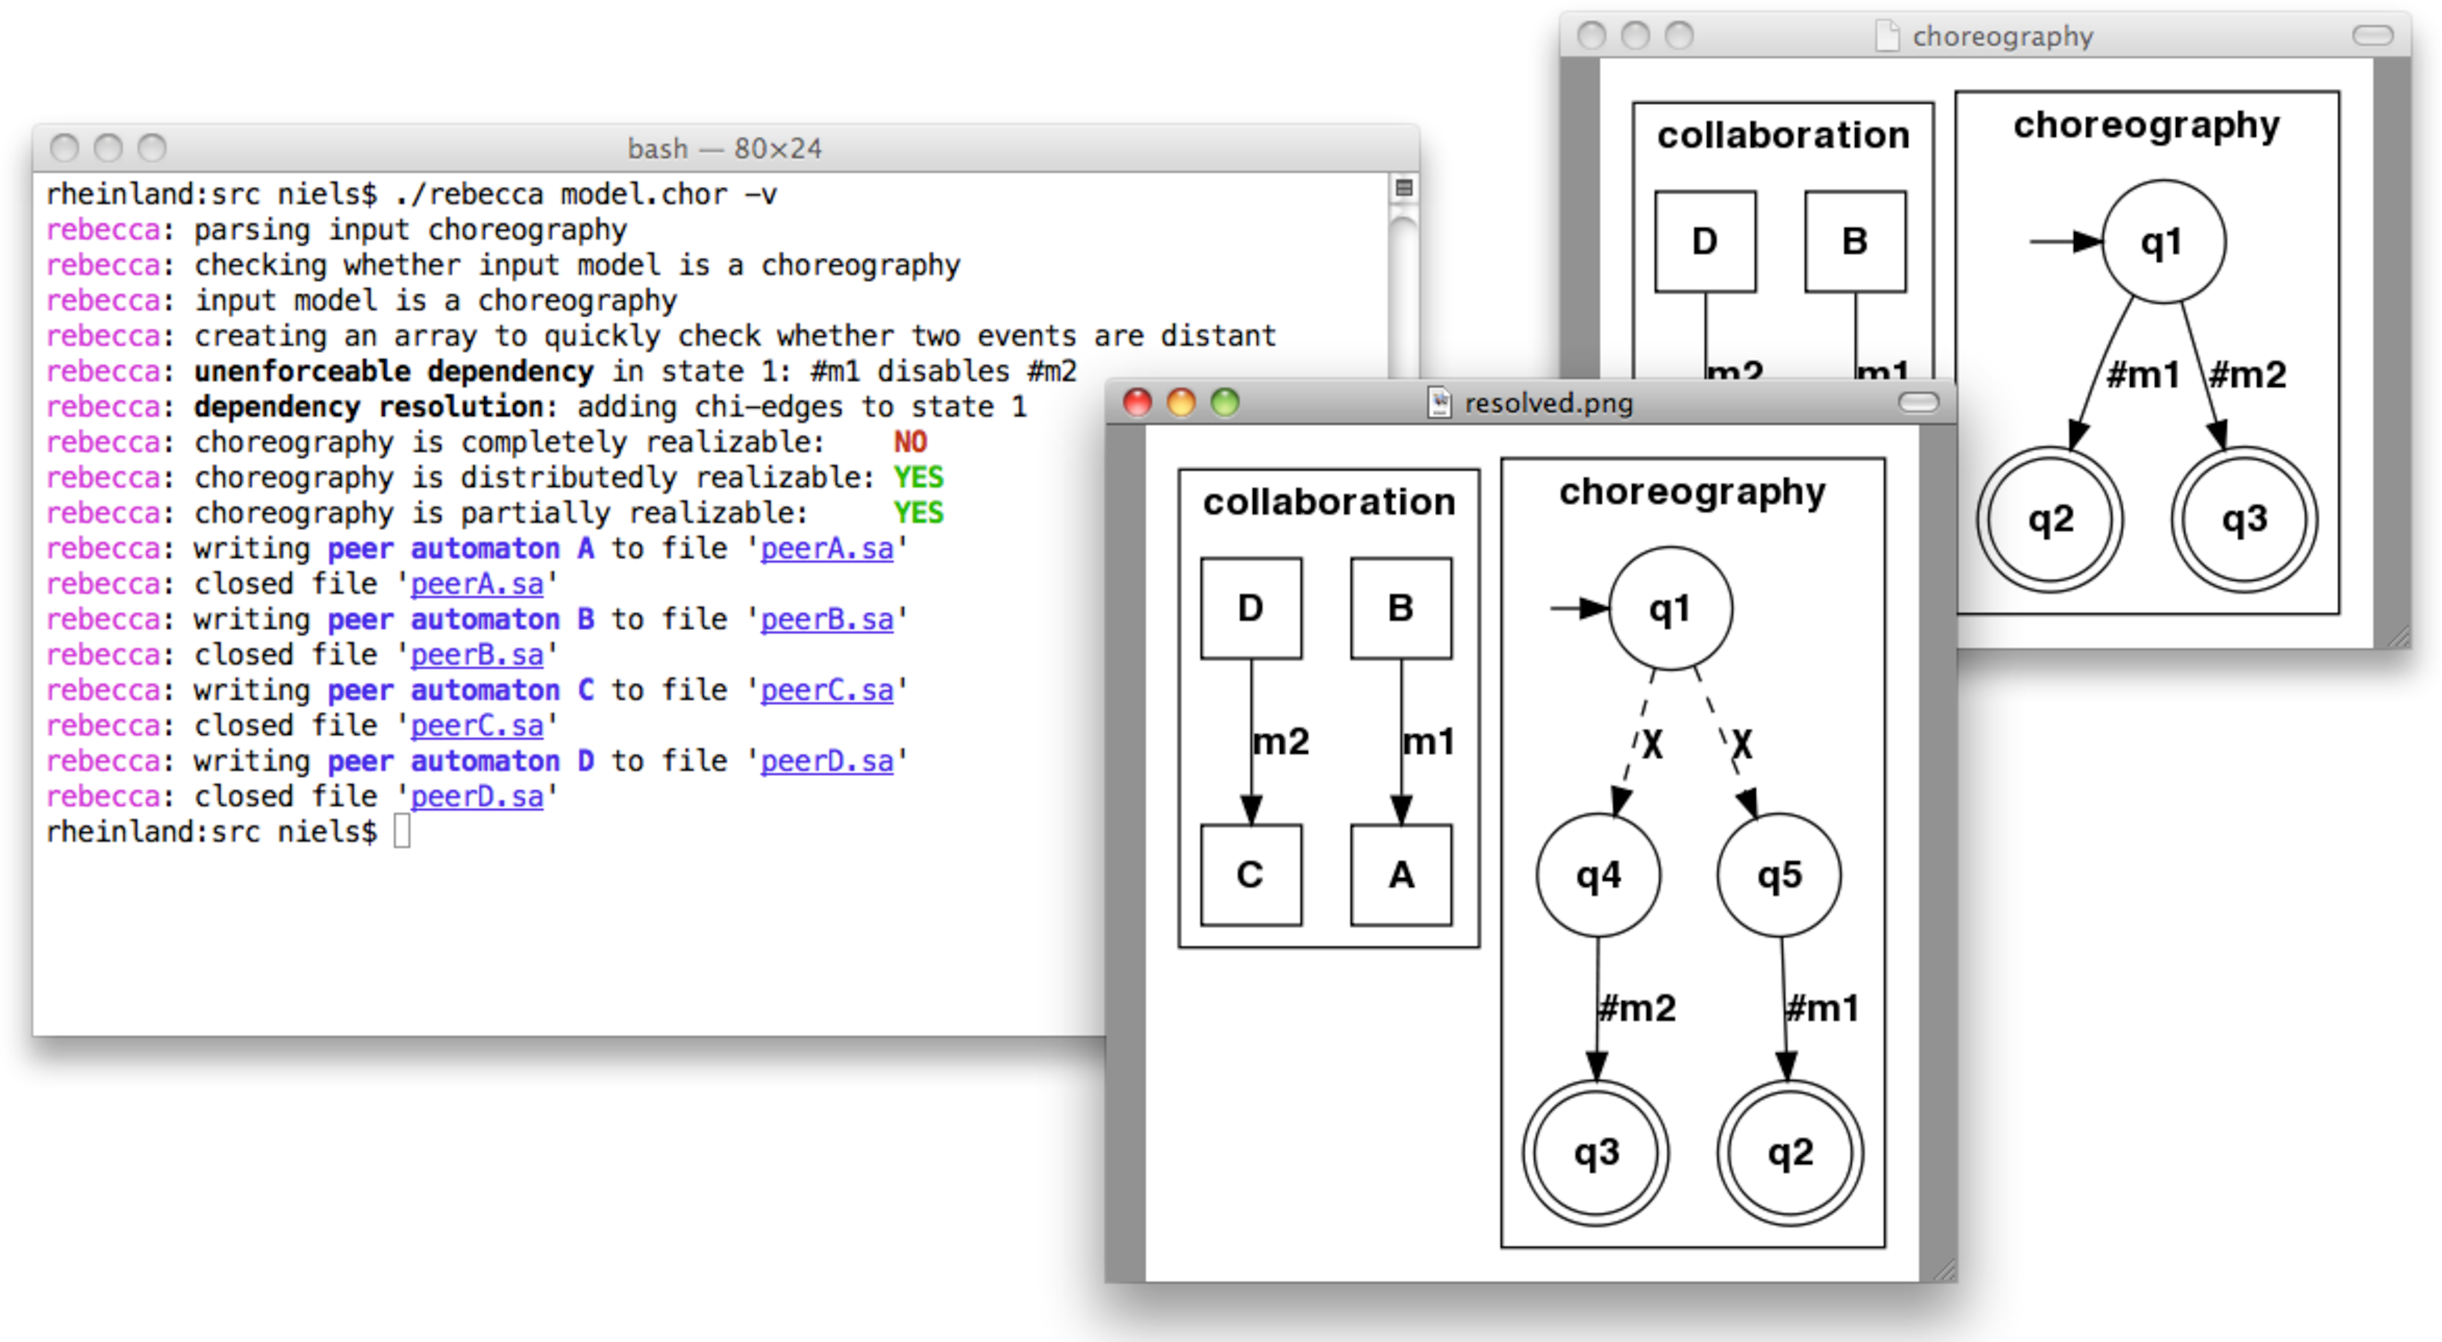
\includegraphics[width=0.8\textwidth]{realizability/rebecca}
\caption{Screenshot of the tool Rebecca analyzing a choreography.}
\end{figure}
%%%%%%%%%%%%%%%%%%%%%%%%%%%%%%%%%%%%%%%%%%%%%%%%%%%%%%%%%%%%%%%%%%%%%%%%%%%%%%



The dependency resolution algorithm and the participant projection has been implemented in a software prototype \emph{Rebecca}~\cite{rebecca}. It analyzes a given choreography specification, resolves dependencies, returns the strongest possible realizability notion, and outputs realizing service automata. We checked various choreography models from literature and it turns out that a lot of models that were unrealizable in a classical sense (\ie, not completely realizable) are in fact distributedly realizable.





%%%%%%%%%%%%%%%%%%%%%%%%%%%%%%%%%%%%%%%%%%%%%%%%%%%%%%%%%%%%%%%%%%%%%%%%%%%%%%%
\section{Realizing asynchronous communication}
\label{sect:realizability_asynchron}
%%%%%%%%%%%%%%%%%%%%%%%%%%%%%%%%%%%%%%%%%%%%%%%%%%%%%%%%%%%%%%%%%%%%%%%%%%%%%%%

Many interaction modeling languages (\eg, \acronym{WS-CDL} or interaction Petri nets) assume atomic and hence synchronous message exchange; that is, the sending and receiving of a message is specified to occur at the same time. Participants realizing such a choreography model inherit this synchronous message model. In implementations, however, asynchronous communication is often preferred over synchronous communication as a ``fire and forget'' send action is more efficient than a blocking handshaking.

To this end, we studied how synchronous peers that realize a choreography can be ``desynchronized''~\cite{DeckerBKL_2008_icsoc}; that is, atomic message exchange is decoupled to a pair of asynchronous send and receive actions. This desynchronization in turn might introduce deadlocks, and the correction toward compatibility results in refinements of the choreography which require domain information and can hardly be automatized. Though the correction approach of \autoref{chap:correction} remains applicable, this would contradict the correctness by construction idea of interaction modeling. \citet{FuBS_2005_tse} propose a reverse approach and study \emph{synchronizability} of choreographies\,---\,a property under which asynchronous communication can be safely abstracted to synchronous communication. Synchronizability can help to detect problems introduced by asynchronous communication, but is only a sufficient criterion and offers only limited support in resolving these issues.

To avoid both restrictions during the design time of a choreography and a later change of the communication model, we used service automata which allow to individually define, for each message, whether it should be transferred in an asynchronous or synchronous manner. We claim that the nature of the message transfer is usually known in an early design phase and helps to refine the choreography model. 

Unlike related work on collaboration diagrams or conversation protocols, we thereby do not just specify the order in which \emph{send} events occur, but also describe the moment of the respective \emph{receive} events. This is crucial to be able to specify dependencies between asynchronous messages. For instance, one is able to express that a customer must not send an order message to a shop before he \emph{received} the terms of payment. If modeled synchronously, the shop would be blocked as long as the customer reads the terms of payment.

In addition, the precise specification of message receipts ensures that the message exchange between the peers can be realized with bounded message buffers. This is  motivated by implementation issues. In addition, unbounded queues would result in an infinite state automaton for which controllability and realizability would be undecidable~\cite{MassutheSSW_2008_ipl}.

In \autoref{def:realizability_choreography}, we restricted choreographies to only consist of conversations. This does not constrain synchronous message events, but only the asynchronous message events. The following definition manipulates an arbitrary closed service automaton such that every terminating run is a conversation; that is, its collaboration language is a choreography. Furthermore, no run will exceed a given message bound $k$. This is done by explicitly taking count of the asynchronous messages on the message channels, and is very similar to the composition of service automata (see \autoref{def:composition}).

%%%%%%%%%%%%%%%%%%%%%%%%%%%%%%%%%%%%%%%%%%%%%%%%%%%%%%%%%%%%%%%%%%%%%%%%%%%%%%
\begin{definition}{\boldmath$k$-bounded service automaton}\label{def:kboundedsa}%
Let $A=[Q,q_{0},{\shortrightarrow},\Omega,\mathcal{P}]$ be a closed $\tau$-free service automaton and $k\in\mathds{N}$. Define the \define{$k$-bounded service automaton} $A_{k}:=[Q',q_{0}',{\shortrightarrow}',\Omega',\mathcal{P}]$ with $Q':=Q\times\mathit{Bags}_{k}(M_{A})$, $q_{0}':=[q_{0},[\,]]$, $\Omega':=\Omega\times\{[\,]\}$ and ${\shortrightarrow}'$ contains exactly the following elements ($\mathcal{B}\in\Bags_{k}(\M_{a})$):
\begin{itemize}
\item $\bigl[[q,\mathcal{B}],\sync x,[q',\mathcal{B}]\bigr]\in{\shortrightarrow}'$ iff \smash{$q\xrightarrow{\sync x}q'$},
\item $\bigl[[q,\mathcal{B}],!x,[q',\mathcal{B}+[x]]\bigr]\in{\shortrightarrow}'$ iff \smash{$q\xrightarrow{!x}q'$} and $\mathcal{B}(x)<k$, and
\item $\bigl[[q,\mathcal{B}+[x]],?x,[q',\mathcal{B}]\bigr]\in{\shortrightarrow}'$ iff \smash{$q\xrightarrow{?x}q'$}.
\end{itemize}
\end{definition}
%%%%%%%%%%%%%%%%%%%%%%%%%%%%%%%%%%%%%%%%%%%%%%%%%%%%%%%%%%%%%%%%%%%%%%%%%%%%%%

The bound $k$ can also be used as a parameter for realizability:

%%%%%%%%%%%%%%%%%%%%%%%%%%%%%%%%%%%%%%%%%%%%%%%%%%%%%%%%%%%%%%%%%%%%%%%%%%%%%%
\begin{definition}{\boldmath$k$-realizability}
Let $C$ be a choreography automaton and $k\in\mathds{N}$. $C$ is (completely/distributedly/partially) \define{$k$-realizable} iff $C_{k}$ is (completely/distributedly/partially) realizable.
\end{definition}
%%%%%%%%%%%%%%%%%%%%%%%%%%%%%%%%%%%%%%%%%%%%%%%%%%%%%%%%%%%%%%%%%%%%%%%%%%%%%%


\paragraph{Example.}

The multiport service automaton of \autoref{fig:realizability_unbounded} did not specify a choreography, because the message buffer for message $x$ is unbounded. Applying \autoref{def:kboundedsa}, we can derive the 2-bounded choreography automaton in \autoref{fig:realizability_boundeda}. The resulting choreography is partially 2-realizable by the service automata in \autoref{fig:realizability_boundedb}.

%%%%%%%%%%%%%%%%%%%%%%%%%%%%%%%%%%%%%%%%%%%%%%%%%%%%%%%%%%%%%%%%%%%%%%%%%%%%%%
\begin{figure}
\centering
\subfigure[2-bounded choreography\label{fig:realizability_boundeda}]{\makebox[0.49\textwidth]{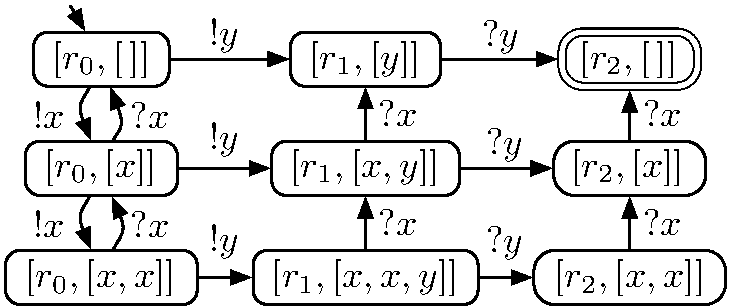
\includegraphics[scale=0.4]{realizability/2chor}}}
\subfigure[partially 2-realizing peers\label{fig:realizability_boundedb}]{\makebox[0.49\textwidth]{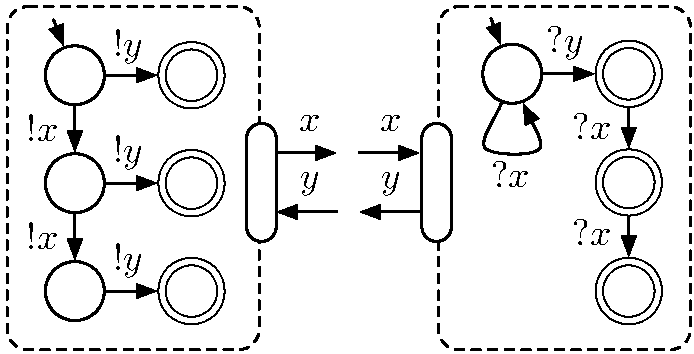
\includegraphics[scale=0.4]{realizability/2peers}}}
\caption{Enforcing a message bound in the choreography of \autoref{fig:realizability_unbounded} to achieve (partial) 2-realizability.}
\label{fig:realizability_bounded}
\end{figure}
%%%%%%%%%%%%%%%%%%%%%%%%%%%%%%%%%%%%%%%%%%%%%%%%%%%%%%%%%%%%%%%%%%%%%%%%%%%%%%





%%%%%%%%%%%%%%%%%%%%%%%%%%%%%%%%%%%%%%%%%%%%%%%%%%%%%%%%%%%%%%%%%%%%%%%%%%%%%%%
\section{Combining interaction models and interconnected models}
\label{sect:realizability_application}
%%%%%%%%%%%%%%%%%%%%%%%%%%%%%%%%%%%%%%%%%%%%%%%%%%%%%%%%%%%%%%%%%%%%%%%%%%%%%%%

We already described the two approaches to model a choreography: The first approach focuses on the interaction between services and uses message exchange events as basic building blocks. These \emph{interaction models} and the corresponding languages such as Let's Dance, \acronym{MSC}s, i\acronym{BPMN} have already been discussed in~\autoref{sect:realizability_framework}. Interaction models are a means to quickly specify a choreography by only modeling the desired observable behavior instead of the local control flow of each participant. With the notion of realizability, these missing local behaviors can then be derived from the choreography. To this end, interaction models are best suited if all peer implementations are unknown. Interaction modeling follows a top-down approach from an abstract global model to concrete participant implementations.

In contrast, the second approach is to specify the choreography implicitly by providing a set of peer implementations and information on their interconnection. As these \emph{interconnected models} specify both the local behavior of the participating services and their interaction, they are close to implementation. Examples of specification languages that follow this modeling style are \acronym{BPMN} and \bpelchor~\cite{DeckerKLW_2007_icws}. Interconnected models aim at reusing existing services in new settings. Though first approaches exist to synthesize individual peers, this modeling style can only be used in a late stage of development, see \autoref{chap:verification}.

However, a setting in which the local behaviors of some peers are completely specified whereas other peers are not specified at all is not supported by any of the  modeling style mentioned. In such a scenario, the completely specified peers can be seen as a constraint of the choreography: The set of all realizing peers is constrained to the set of those peers that not only realize the choreography, but are also compatible to the completely specified peers. By using service automata as uniform formalism to model both choreographies and peer implementations, we can support this mixed scenario as follows.

The choreography specifies the global interaction of all peers, whereas a completely specified peer only specifies its local communication protocol. The service automaton describing this protocol can be transformed into a constraint automaton (see \autoref{def:constraint}) be replacing each $x$-labeled transition with a transition that is labeled with the set of all $x$-labeled transition of the choreography automaton. The product of the choreography automaton and this constraint automaton is then a multiport automaton whose terminating runs are conversations of the choreography and than can be projected to terminating runs of the service automaton. This multiport automaton can then be transformed into a choreography automaton by removing all deadlocking states and by collapsing all $\tau$-transitions. The latter operation is standard for finite automata~\cite{HopcroftMU_1979} and preserves the language of the automaton. The resulting choreography automaton can then be analyzed as before.

A combination of classical \acronym{BPMN} constructs together with i\acronym{BPMN} extensions~\cite{DeckerB_2007_bpmw} (\ie, modeling processes both inside and and outside pools) could be used to present this mixed choreography modeling approach to modelers with a unique graphical representation. The combination of both modeling approaches is also supported the recent standard of \acronym{BPMN}~2.0~\cite{standard_bpmn2}.

%%%%%%%%%%%%%%%%%%%%%%%%%%%%%%%%%%%%%%%%%%%%%%%%%%%%%%%%%%%%%%%%%%%%%%%%%%%%%%
\begin{figure}[t!]
\centering
\subfigure[choreography]{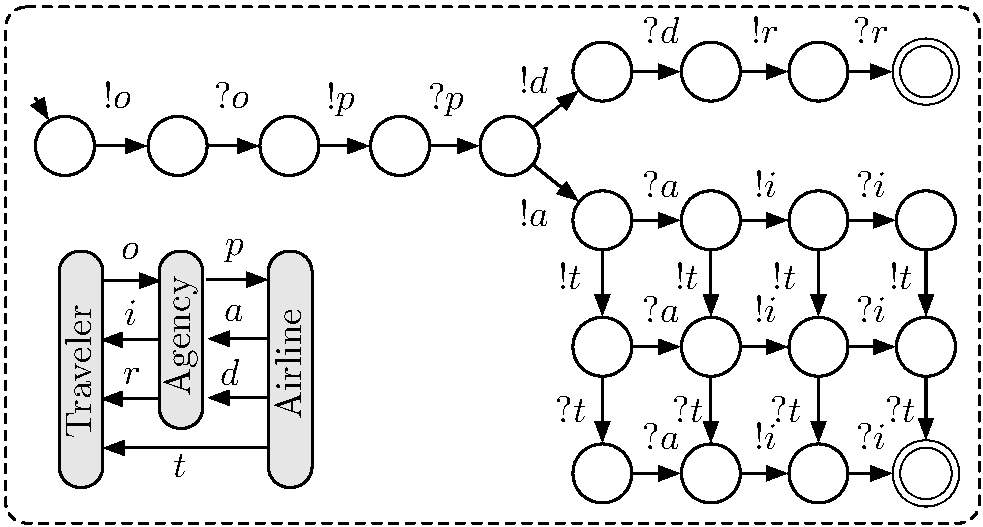
\includegraphics[scale=0.4]{realizability/bigex1}}
\subfigure[completely realizing service automata]{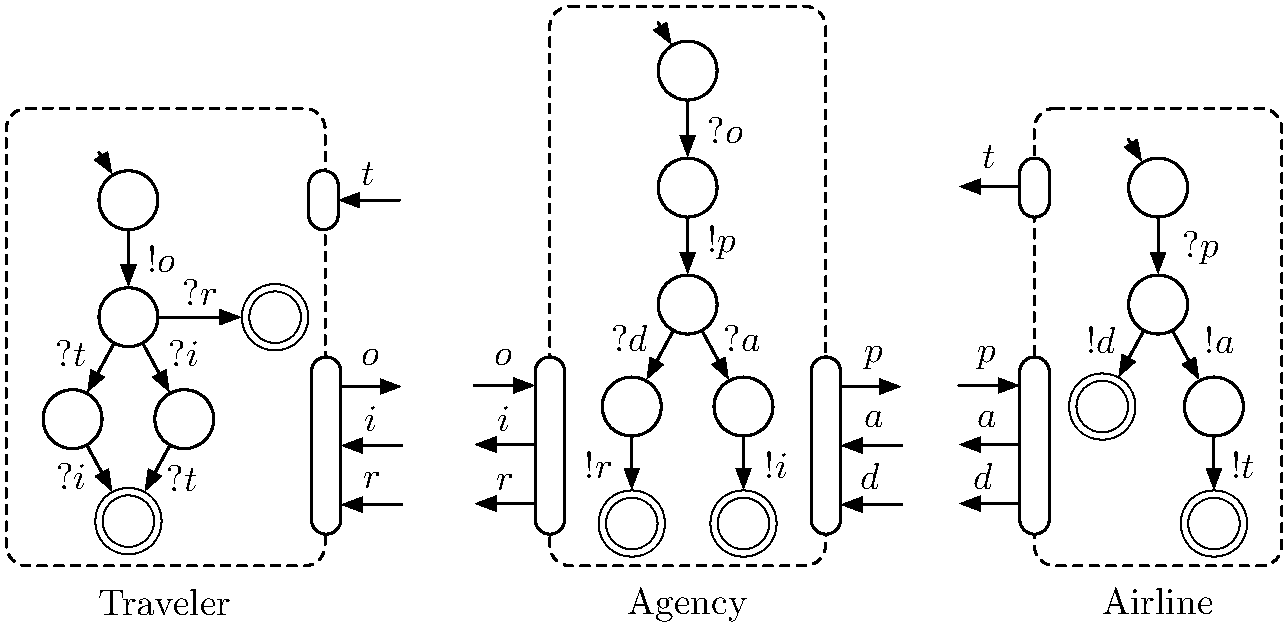
\includegraphics[scale=0.4]{realizability/bigex2}}\\
\subfigure[implemented service]{\makebox[0.3\textwidth]{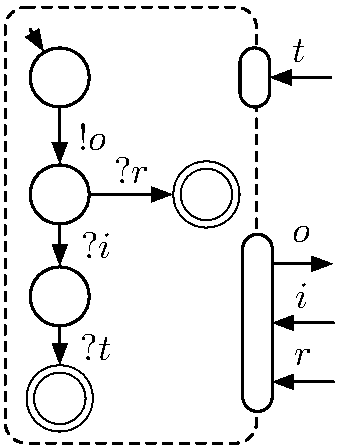
\includegraphics[scale=0.4]{realizability/bigex3}}}\hfill
\subfigure[constrained choreography]{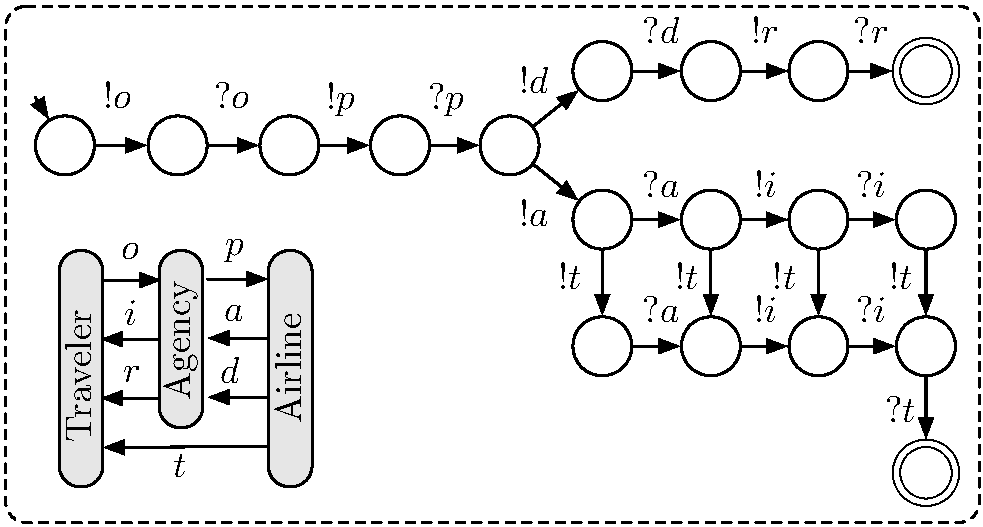
\includegraphics[scale=0.4]{realizability/bigex4}}
\caption{Combination of choreography models.}\label{fig:realization:combination}
\end{figure}
%%%%%%%%%%%%%%%%%%%%%%%%%%%%%%%%%%%%%%%%%%%%%%%%%%%%%%%%%%%%%%%%%%%%%%%%%%%%%%


\paragraph{Example.}

\Autoref{fig:realization:combination} sketches an example for the proposed combination of choreography models. The observable behavior of a simplified version of the traveler example (cf.\ \autoref{fig:fixed}) is given as choreography automaton (a). It specifies the interplay between a traveler that sends an order ($o$) to a travel agency which quotes a price ($p$) from an airline. The airline can either accept ($a$) or declines ($d$) the booking. In the former case, the traveler receives an itinerary ($i$) from the travel agency and a ticket ($t$) from the airline. In the latter case, only a rejection ($r$) message is sent. This choreography can be completely realized (b). The realizing service automaton of the traveler can receive the itinerary and the ticket in any order. 

Now assume that instead of the realized service automaton, an already implemented traveler service~(c) with more restricted behavior should be used in the service composition under design. This service automaton can be used as a constraint to the choreography specification, yielding a constrained choreography~(d) in which the invoice is always received before the ticket.





%%%%%%%%%%%%%%%%%%%%%%%%%%%%%%%%%%%%%%%%%%%%%%%%%%%%%%%%%%%%%%%%%%%%%%%%%%%%%%%
\section{Related Work}\label{sect:realizability_related}
%%%%%%%%%%%%%%%%%%%%%%%%%%%%%%%%%%%%%%%%%%%%%%%%%%%%%%%%%%%%%%%%%%%%%%%%%%%%%%%

Realizability received much attention in recent literature, and was studied for most of the aforementioned interaction modeling languages, see \cite{SuBFZ_2007_wsfm} for a survey. Note that the term realizability as used in this thesis focuses on service choreographies. The classical notion of realizability is tightly linked to program/process synthesis from logical specification, see, for instance,~\cite{Vardi_2008_25mc}. Beside the different specification languages, the approaches differ in (1)~the expressiveness of the specification language (the main differences concern the support of arbitrary looping) and (2)~the nature of the message exchange (synchronous vs.\ asynchronous) of the realizing peers. In the following, we classify related approaches into these two groups.


\paragraph{Structural restrictions.}

\citet{AlurEY_2003_tse} present necessary and sufficient criteria to realize a choreography specified by a set of message sequence charts (\acronym{MSC}s) with a set of concurrent automata. Both synchronous and asynchronous forms of communication are supported. Their proposed algorithms are very efficient, but are limited to acyclic choreography specifications, because the \acronym{MSC} model used in the paper does not support arbitrary iteration which excludes models such as \autoref{fig:realizability_resolvec}.

\citet{SalaunB_2009_ifm} investigate complete and partial realizability of choreographies specified by collaboration diagrams. The authors express the realizability problem in terms of \acronym{LOTOS} and present a case study conducted with a \acronym{LOTOS} verification tool. Their approach tackles both synchronous and asynchronous communication (using bounded \acronym{FIFO} queues). Collaboration diagrams, however, provide only limited support for repetitive behavior (only single events can be iterated and cycles such as in \autoref{fig:realizability_resolvec} cannot be expressed) and choices (events can be skipped, but complex decisions cannot be modeled). These restrictions also apply to~\cite{BultanF_2008_soca} in which sufficient conditions for complete realizability of collaboration diagrams are elaborated. A tool to check the sufficient criteria of~\cite{BultanF_2008_soca,FuBS_2004_tcs,FuBS_2005_tse} is presented by~\citet{BultanFF_2009_icws}. Using this tool, the authors showed that many collaboration diagrams in literature are unrealizable.


\paragraph{Communication models.}

Realizability of conversation protocols by asynchro\-nously communicating B\"uchi automata is examined by \citet{FuBS_2004_tcs}. The authors show decidability of the problem and define a sufficient condition for complete realizability. One of the prerequisites, \emph{synchronous compatibility}, heavily restricts asynchronous communication.

Algorithms to check choreographies for partial realizability are discussed by \citet{ZahaDHBD_2006_edoc}. Both the global and local model are specified in Let's Dance and only atomic message exchanges considered. \citet{DeckerW_2007_bpm} study realizability of interaction Petri nets. To the best of our knowledge, it is the only approach in which (complete and partial) realizability is not defined in terms of complete trace equivalence (cf.\ \autoref{def:realizability_completerealizability}). Instead, the authors require the participant implementations and the choreography to be branching bisimilar. Message exchange specified by interaction Petri nets is, however, inherently synchronous.

\citet{KazhamiakinP_2006_forte} study a variety of communication models and their impact on realizability. They provide an algorithm that finds the ``simplest'' communication model under which a given choreography can be completely realized. Their approach is limited to complete realizability and gives no diagnosis information in case the choreography cannot be implemented by participants. Furthermore, they fix the communication model for all messages instead of allowing different communication models for each message.


\paragraph{Other aspects.}

For other issues of choreographies such as instantiation, reference passing, or compliance checking, verification techniques are available for Let's Dance~\cite{DeckerZD_2006_wsfm}) and \acronym{WS-CDL}~\cite{BusiGGLZ_2006_coordination,Angelis_2007_yrsoc}. \citet{AlurEY_2005_tcs} report decidability results in context of \acronym{MSC} graphs.

\citet{McIlvennaDW_2009_apccm} describes an approach to derive an orchestrator service from a service choreography given as interconnected model. This orchestrator is motivated by possible added value and flexibility for the participating services rather than by choreography verification.

Declarative modeling of choreographies is studied by~\citet{MontaliPACMS_2009_tweb}. The authors compare declarative models with interconnected models and report several advantages of the former modeling style. In particular, a declarative model does not necessarily be closed, but additionally constraints can be easily added. Furthermore, such a model is guaranteed to specify maximal behavior. However, the question how to realize a declarative choreography model by local service implementation is not addressed yet.

\bigskip

The original contribution is an automaton framework to specify arbitrary regular choreographies, check for various realizability notations, and to synthesize participants services that implement as much behavior as possible. There\-by, it is possible to define the message model individually for each message. Additionally, the defined synthesis algorithm provides diagnosis information that can help to fix choreographies toward complete realizability.





%%%%%%%%%%%%%%%%%%%%%%%%%%%%%%%%%%%%%%%%%%%%%%%%%%%%%%%%%%%%%%%%%%%%%%%%%%%%%%%
\section{Conclusion}\label{sect:realizability_conclusion}
%%%%%%%%%%%%%%%%%%%%%%%%%%%%%%%%%%%%%%%%%%%%%%%%%%%%%%%%%%%%%%%%%%%%%%%%%%%%%%%

In this chapter, we linked the realizability problem of choreographies to the controllability problem of orchestrations. The close relationship between orchestrations and choreographies on the one hand and controllability and realizability on the other hand has been anticipated before: \citet{PapazoglouTDL_2007_ieee} sketch a research road map for service-oriented computing. On service orchestrations and service choreographies, they comment:
\begin{quote}
This sharp distinction between orchestration and choreography is rather artificial, and the consensus is that they should coalesce in a single language and environment.
\end{quote}
\citet{DumasBN_2008_deb} review related notions for services such as realizability, substitutability and controllability. Substitutability can be realized with operating guidelines and is hence naturally related to controllability. However:
\begin{quote}
The problem of controllability is intuitively related to that of realizability\,---\,as that they both result when internal choices are not externalized as messages. However, a formal relation between controllability and realizability is yet to be established.
\end{quote}

The close relationship between these problems offers a uniform way to analyze and model arbitrary interacting services.  Hence, we were able to reuse techniques that were originally proposed to check for controllability. These techniques resulted in a formal framework that allows to specify and analyze choreographies with both synchronous and asynchronous communication. Realizing choreographies offers a \emph{correctness-by-construction} alternative to the composition of existing services: Compatibility of the realized peers follows from the realizability algorithm rather than from an a posteriori check. In addition, we refined the existing hierarchy of realizability notions by defining the novel notion of distributed realizability. Finally, we proposed to combine interaction models and interconnected models.

\medskip

By reducing realizability to decentralized controllability, we also inherited the limitations of the synthesis algorithm. That is, we currently cannot guarantee that the algorithm sketched in \autoref{def:realizability_resolution} always terminates for cyclic choreography models. This is subject of future work. The introduction of $\chi$-arcs allows us to resolve dependencies without deleting states. The resulting service automaton can be seen as a most-permissive strategy for decentralized controllability. In future work, we need to study the step toward a finite representation of decentralized strategies; that is, a decentralized operating guideline.

Finally, further consequences of the relationship between controllability and realizability need to be examined. For instance, controllability is used in several other applications such as test case generation~\cite{KaschnerL_2008_wesoa} or service mediation~\cite{GierdsMW_2010_tcs}. We expect these techniques to be similarly applicable to choreographies.
